\chapter{Analysis of Gamification in Language Learning Applications}

The motivation behind gamifying vocabulary learning is to increase learning efficiency and long-term retention through the inclusion of game elements that increase user motivation and engagement. Traditional methods of vocabulary learning, such as mechanical repetition or passive reading, can often be monotonous and lead to a decline in interest. Gamification brings these methods to life through elements such as rewards, challenges and competitions, leading to higher intrinsic learner's motivation.

By using gamification mechanisms it is possible to create an environment that is not only more interesting for students but also encourages repeated and focused learning. In this way, the student might remember the vocabulary better, not only on a short-term basis, but especially in the long term, which is one of the main goals of vocabulary learning.

Gamification encompasses a vast array of concepts, including streaks, badges, achievements, challenges, quests, leaderboards, rewards, statistics, progression tracking, levels and tiers, user-generated content, time-limited events, feedback loops, personalization, social elements, narrative and storytelling, virtual currencies, and so on. Furthermore, all of them can be combined and mixed in various ways. Therefore, we will focus on a selected few that can significantly enhance the user experience in the English Mind app rather than trying to cover every single gamification concept that could benefit vocabulary learning.

\textbf{TODO: add citation, add in the following sections we will analyze....}

\section{Current Gamification in English Mind}

English Mind currently lacks extensive gamification features, relying instead on a few elements that can be classified as basic forms of gamification. We have identified three such elements:

\begin{itemize}
    \item \textbf{Progress Tracking of Vocabulary Acquisition} 
    \label{chap:em-progess-tracking-of-vocabulary-aquisition}
    
    Users can view essential statistics regarding their vocabulary acquisition, including the number of words they already know, the number they are currently learning, and the total remaining words to uncover. These statistics are accessible on both the vocabulary levels overview screen and on the specific vocabulary level screen.

    \begin{figure}[!h]
        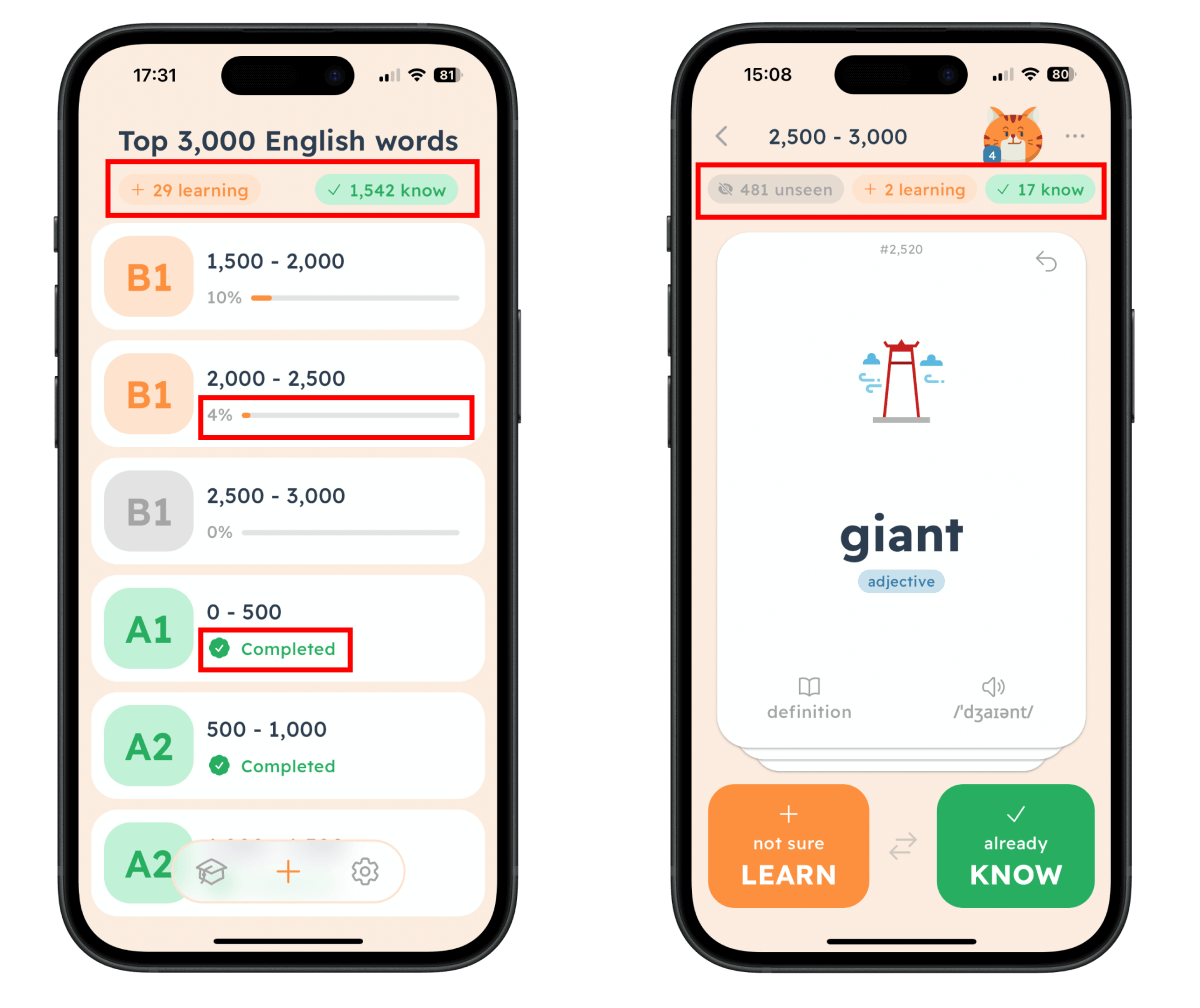
\includegraphics[width=0.65\textwidth]{src/figures/em-progress-tracking.png}
        \caption{English Mind - Progress Tracking of Vocabulary Acquisition (highlighted in red)}
        \label{fig:em-progress-tracking}
    \end{figure}

    \item \textbf{Daily Goal}
    
    During an onboarding process, users set a personal goal for the number of new words they wish to learn or add each day.

    Additionally, a mascot appears in the top right corner on the word addition screen to count the newly added words awaiting their first practice session (see Figure \ref{fig:em-daily-goal}). This mascot serves a dual purpose, it tracks word additions and helps ensure that users do not overwhelm themselves by adding too many new words to learn at once.

    \begin{figure}[!h]
        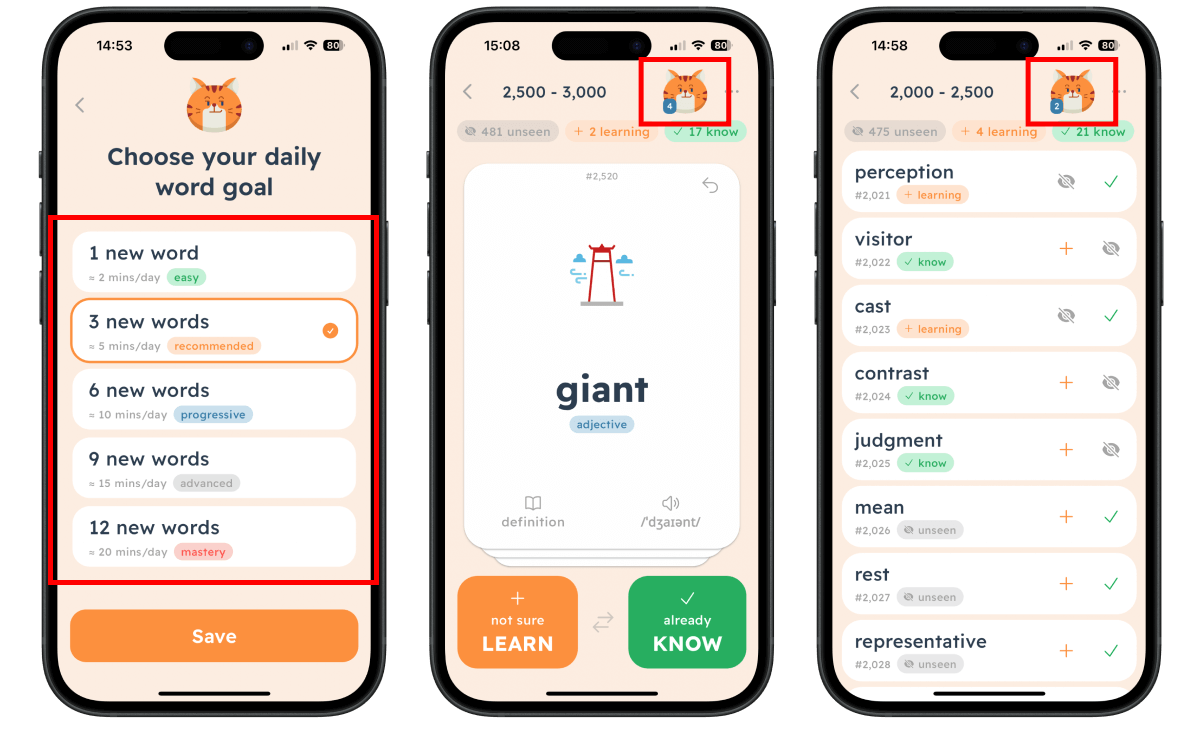
\includegraphics[width=0.8\textwidth]{src/figures/em-daily-goal.png}
        \caption{English Mind - Daily Goal and Word Addition Tracker (both highlighted in red)}
        \label{fig:em-daily-goal}
    \end{figure}

    \newpage

    \item \textbf{Progress Bar}
    
    While learning vocabulary through the daily queue of flashcards, users are presented with a progress bar that visually indicates their advancement, which gives them instant feedback as they progress and might motivate them to finish the current daily queue of flashcards (see Figure \ref{fig:em-flashcards-progress-bar}). Although this is a minor gamification feature, it is noteworthy given the app’s limited implementation of gamification elements.

    \begin{figure}[!h]
        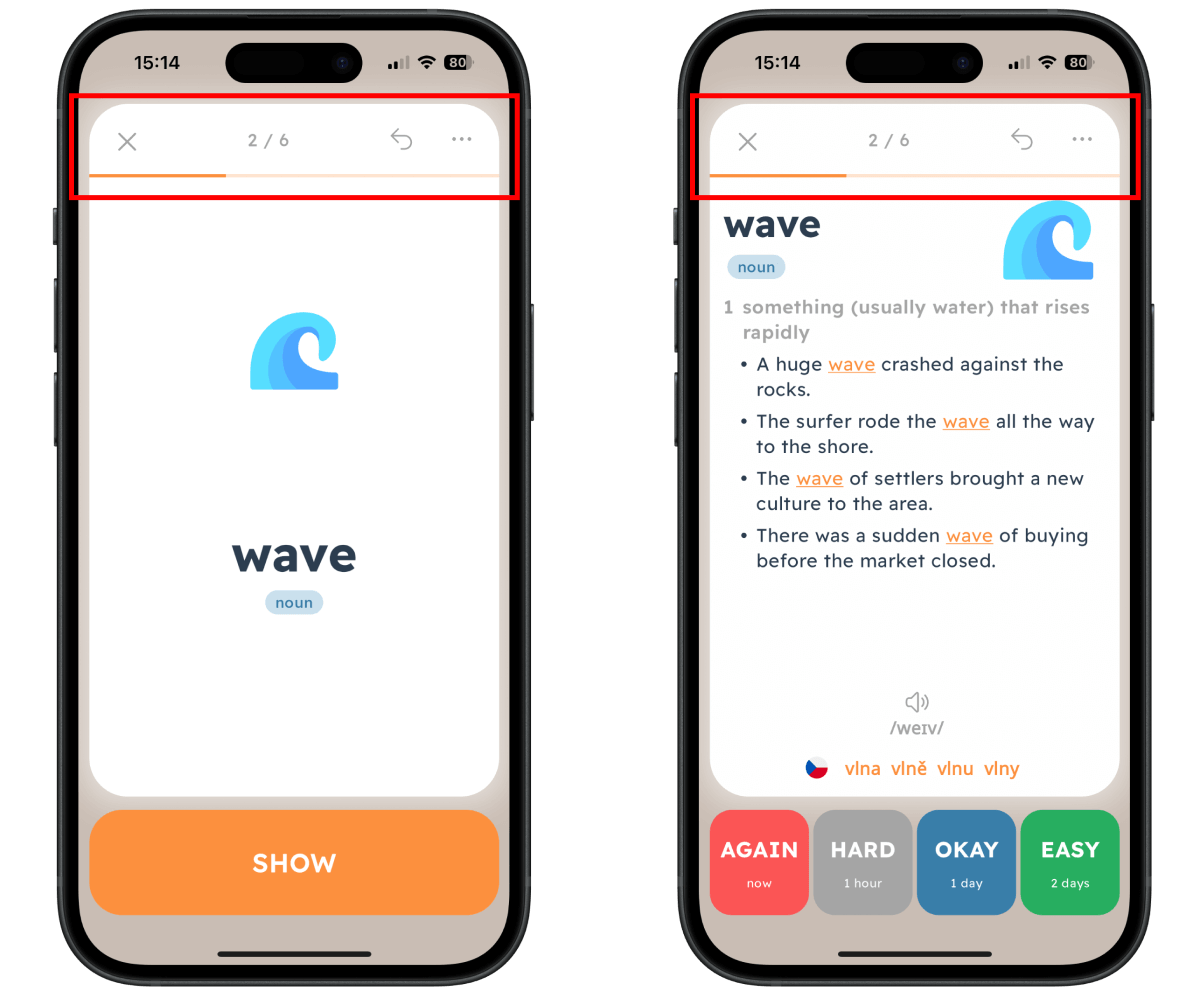
\includegraphics[width=0.65\textwidth]{src/figures/em-flashcards-progress-bar.png}
        \caption{English Mind - Progress Bar (highlighted in red)}
        \label{fig:em-flashcards-progress-bar}
    \end{figure}
    
\end{itemize}

In summary, there is potential to enhance the app by developing a more comprehensive gamification framework, which could further enrich the user experience and encourage greater motivation for improved learning outcomes.

\section{Gamification in Similar Applications}

Before proposing new gamification features for the English Mind app, we decided to briefly analyze three mobile apps that either closely align with its learning concepts, as discussed in Chapter \ref{chap:mobile-application-english-mind}, or demonstrate innovation in the field of gamification. The selected applications are: 

\begin{itemize}
    \item \textbf{WordUp} \cite{cite:wordup}

    This app closely resembles English Mind in terms of learning concepts, as it also combines flashcards with frequency lists and a spaced repetition system.

    \item \textbf{DuoCards} \cite{cite:duocards}

    DuoCards is similar to English Mind, utilizing both flashcards and a spaced repetition system, but it lacks the incorporation of frequency lists.

    \item \textbf{Duolingo} \cite{cite:duolingo}

    While Duolingo is not based on the same learning concepts as English Mind, it was chosen for its extensive use of gamification elements and its innovations in the field. These features offer valuable inspiration for potential enhancements.
    
\end{itemize}

The following subsections will briefly explore the gamification elements used in each of these apps.

\subsection{WordUp}

WordUp application is particularly relevant as it utilizes the same learning concepts as English Mind and could inspire new gamification strategies that further support and enhance these concepts. The app has over 5 million downloads on Google Play with an average rating of 4.5 stars \cite{cite:wordup_google_play}, making it one of the most downloaded apps in English language learning field.

The app's gamification analysis identified relatively fewer gamification features despite its popularity. The vast majority of the elements identified were related in some way to practicing the flashcards queue. In the area of adding new words, a single gamification element was identified. Namely, the progress completion of a particular vocabulary range, which is very similar to the \textit{progress tracking of vocabulary acquisition} \ref{chap:em-progess-tracking-of-vocabulary-aquisition} in English Mind; therefore, it will not be listed.

Identified gamification elements are:

\begin{itemize}
    \item \textbf{Various Types of Flashcards}

     WordUp uses four different types of flashcards that are rotated regularly to break the stereotype of flashcard practice. Each flashcard type focuses on a different aspect of learning acquisition or its combination, such as meaning, spelling, and listening. This approach effectively mitigates the monotony often associated with traditional flashcard practice, thereby increasing user engagement and interest. The four types of flashcard are (see Figure \ref{fig:wordup-flashcard-types}):
    
    \begin{itemize}
        \item \textbf{Read a word and choose the correct definition}
        
        Promotes word comprehension by having users select the most accurate definition, reinforcing meaning and usage.
        
        \item \textbf{Read a definition and choose the correct word}

        Strengthens recall by prompting users to match the definition with the correct term.
        
        \item \textbf{Read a definition and choose the correct spelling}

        This type emphasizes spelling accuracy, requiring users to focus on the correct letter sequence while associating the word with its meaning.
        
        \item \textbf{Listen to a word and choose the correct spelling}

        Enhances auditory skills and spelling, as users select the correct spelling of the spoken word.
        
    \end{itemize}

    \begin{figure}[!h]
        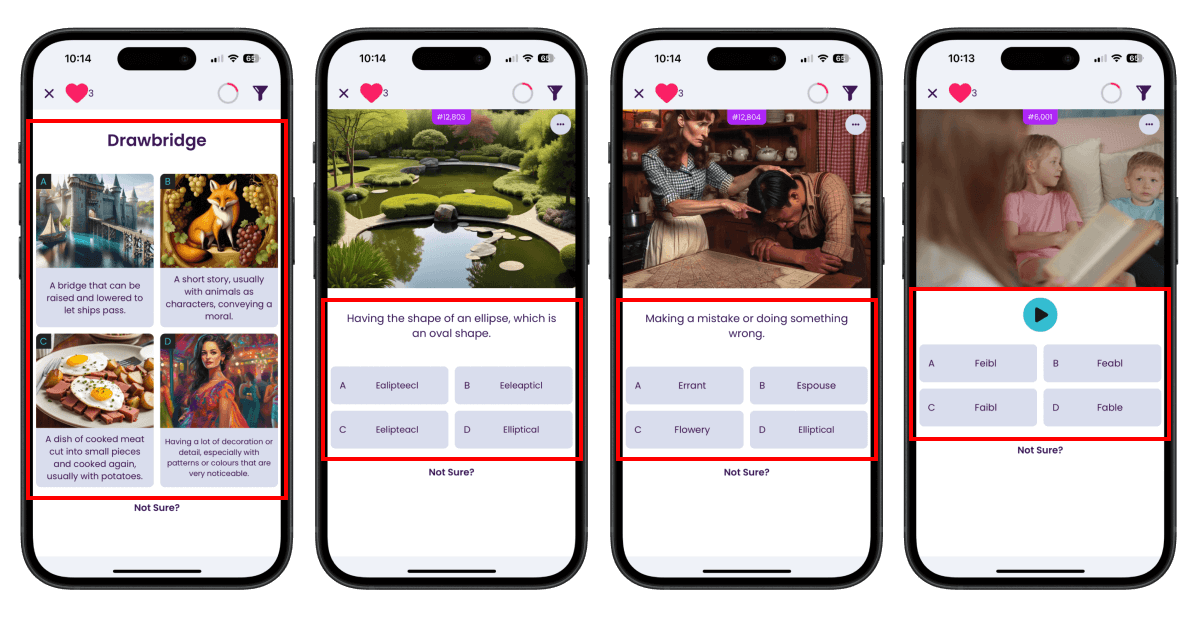
\includegraphics[width=1\textwidth]{src/figures/wordup-flashcard-types.png}
        \caption{WordUp - Types of Flashcards (highlighted in red)}
        \label{fig:wordup-flashcard-types}
    \end{figure}
    
    \item \textbf{Progress tracking for individual words}
    
    WordUp uses its own unique spaced repetition system. It features a visual indicator that tracks each word's progress, showing how many times the user has correctly recalled it (see Figure \ref{fig:wordup-word-progress}). This interactive feedback motivates continued practice, rewarding users with a sense of achievement as they advance.

    \begin{figure}[!h]
        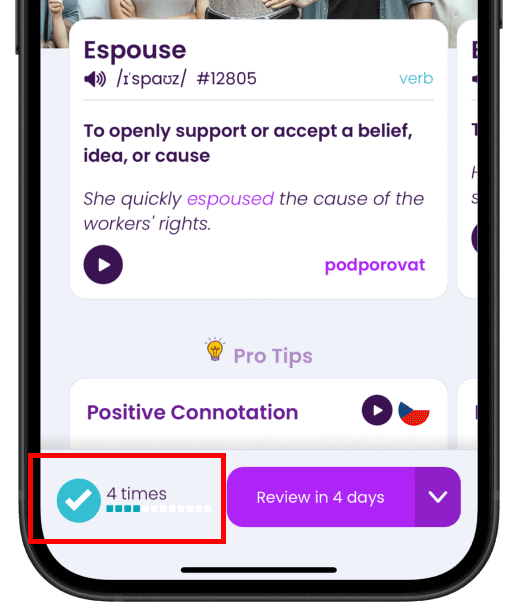
\includegraphics[width=0.35\textwidth]{src/figures/wordup-word-progress.png}
        \caption{WordUp - Indicator of Word's Progress (highlighted in red)}
        \label{fig:wordup-word-progress}
    \end{figure}

    \item \textbf{Daily Goal and Leaderboard}

    WordUp introduces a daily goal based on minutes spent practicing to motivate users to practice regularly. First, the user sets a daily commitment for how many minutes they intend to practice English vocabulary. Each day, they strive to complete a circular progress ring representing this goal, providing a clear sense of accomplishment (see Figure \ref{fig:wordup-daily-goal}).
    
    Additionally, WordUp includes a leaderboard that ranks users based on the minutes they spend practicing (see Figure \ref{fig:wordup-daily-goal}). Users can compare their achievements with friends or other learners, adding a social and competitive element that encourages continued practice. 

    \begin{figure}[!h]
        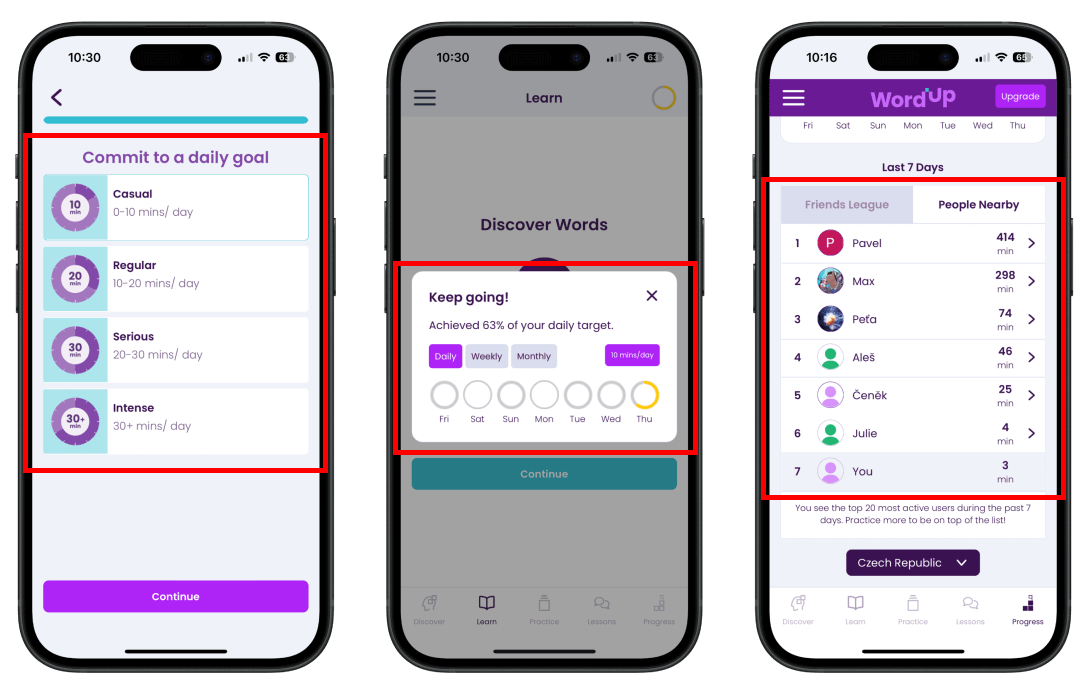
\includegraphics[width=0.99\textwidth]{src/figures/wordup-daily-goal.png}
        \caption{WordUp - Daily Goal and Leaderboard (both highlighted in red)}
        \label{fig:wordup-daily-goal}
    \end{figure}

\end{itemize}

\subsection{DuoCards}

The DuoCards application uses an SRS-based flashcard approach for vocabulary practice and has over a million downloads on Google Play with an average rating of 4.6 stars \cite{cite:duocards_google_play}. 

The analysis of gamification features reveals two key concepts: various types of flashcards and a more complex mascot upgrade system using virtual currency. The following sections provide detailed descriptions of these two concepts.

\begin{itemize}
    \item \textbf{Various Types of Flashcards}

    Duocards utilizes four different types of flashcards (see Figure \ref{fig:duocards-flashcard-types}) to keep practice exciting and address various aspects of language acquisition, such as spelling and meaning. This gamified approach maintains user interest, enhancing the learning experience. Identified flashcard variants are:

    \begin{itemize} 
         \item \textbf{English to Native Language}
         
         Displays an English word on the front, with its translation on the back. 

         \item \textbf{Native Language to English}
         
         Reverses the direction, showing the native language word on the front and prompting the English translation on the back.
         
        \item \textbf{Pronunciation Focus}
        
        Emphasizes auditory learning by presenting only the word’s pronunciation, with spelling revealed upon flipping the flashcard. 
        
        \item \textbf{Matching Exercise}
        
        Appears periodically, involving the matching of five words with their correct translations. 
    
    \end{itemize}

    \begin{figure}[!h]
        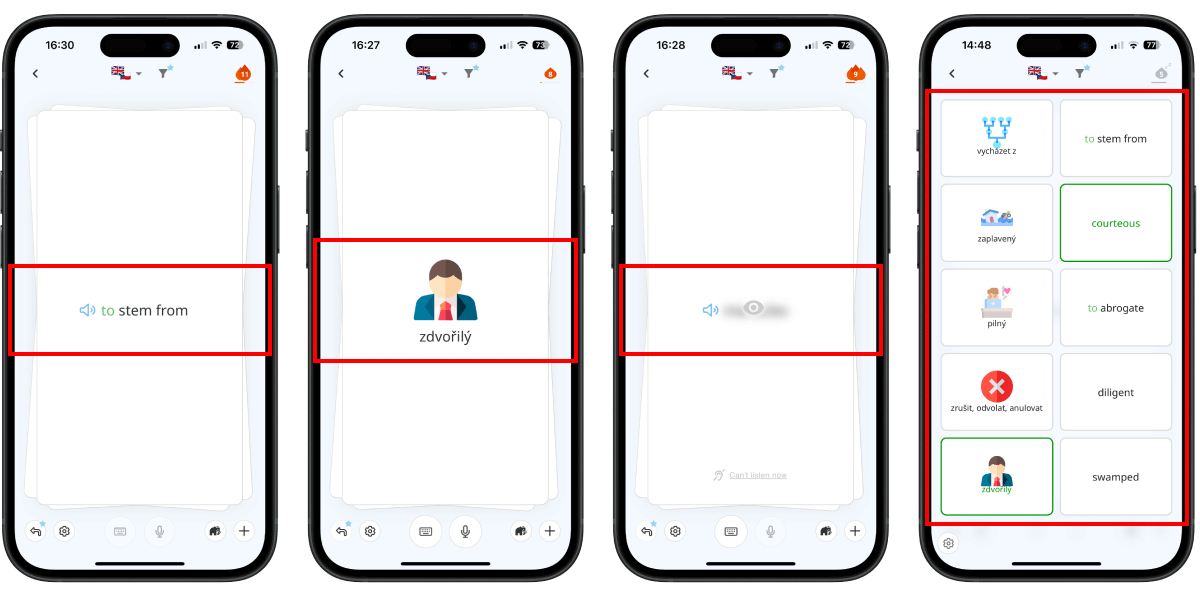
\includegraphics[width=0.98\textwidth]{src/figures/duocards-flashcard-types.png}
        \caption{DuoCards - Types of Flashcards (highlighted in red)}
        \label{fig:duocards-flashcard-types}
    \end{figure}
    
    \item \textbf{Mascot Upgrade System and Virtual Currency}

    The app’s most intriguing gamification feature is its mascot, Memo, which lives in a customizable habitat on the main screen. Users can upgrade Memo’s home by purchasing and arranging various items, creating a personalized space for them. These upgrades require a virtual currency, XP (Experience Points), which users earn by practicing and adding new vocabulary. This system rewards learning progress and adds a creative, interactive layer to vocabulary practice.

    By engaging users in developing Memo’s habitat, the app stimulates a sense of ownership and investment in the learning process. This connection can enhance motivation and commitment to vocabulary acquisition, making learning feel more like a game than a chore. 

    \begin{figure}[!h]
        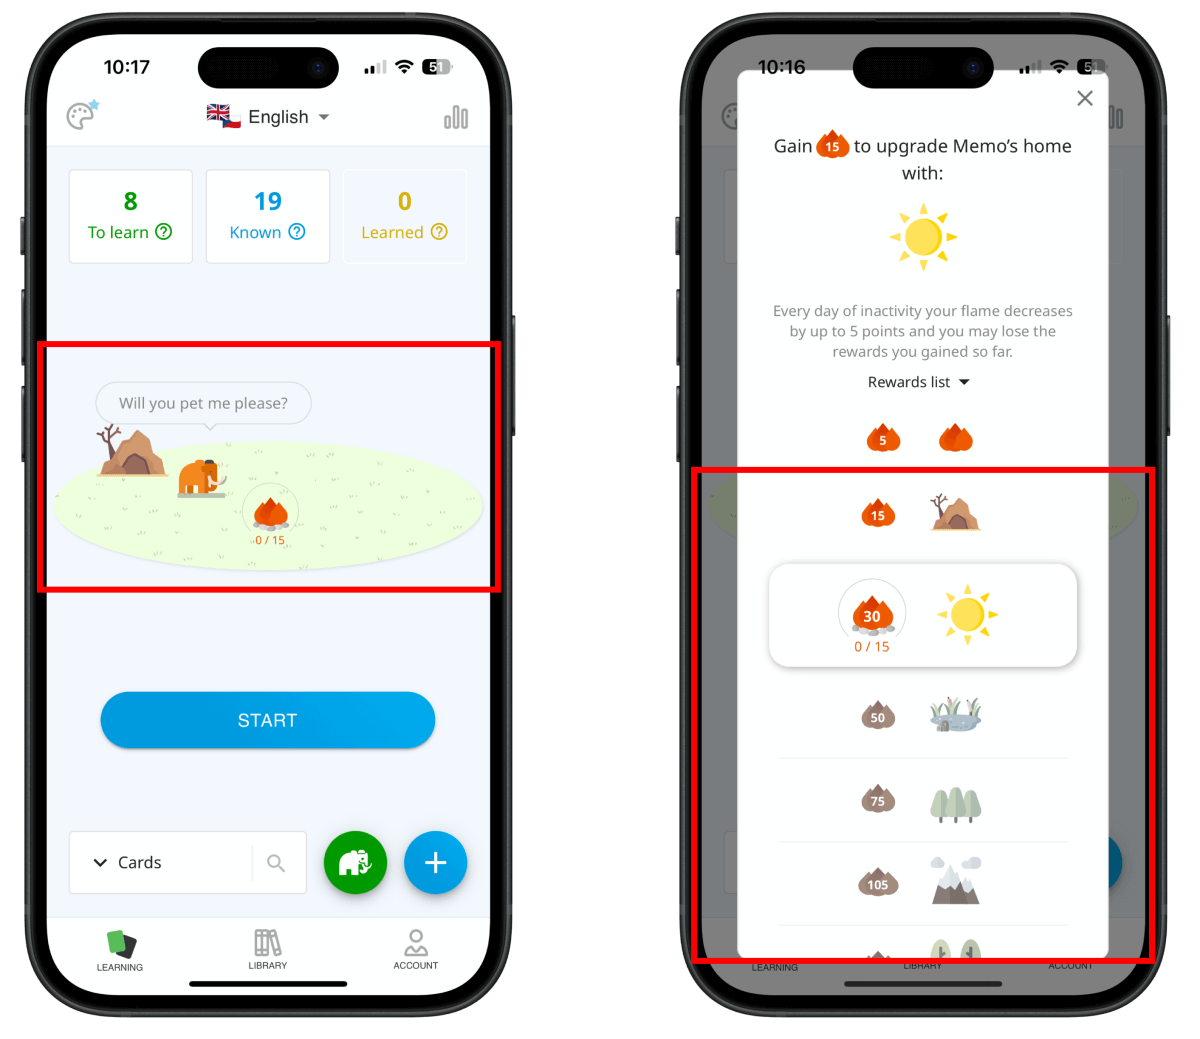
\includegraphics[width=0.7\textwidth]{src/figures/duocards-memo.png}
        \caption{DuoCards - Mascot Upgrade System (highlighted in red)}
        \label{fig:duocards-memo}
    \end{figure}

\end{itemize}

\subsection{Duolingo}

Duolingo, the world's most popular language learning application with over 100 million monthly active users \cite{cite:duolingo_2024q2}, has revolutionized digital language education through its accessible and engaging approach. The application was chosen for analysis due to its pioneering innovations in gamification. While numerous studies have examined Duolingo's gamification strategies, we will focus only on a few elements that could be effectively adapted for English Mind, particularly those that complement its learning concepts and methodologies.

Analysis revealed three concepts that English Mind could benefit from if implemented effectively. The following sections provide an introduction to these concepts.

\begin{itemize}
    \item \textbf{Various Exercises}

    Duolingo structures its content into bite-sized lessons, each consisting of a series of varied exercises similar to interactive flashcards. The variety of exercises keeps users engaged as they practice. Some of these exercises include:

    \begin{itemize}
        \item \textbf{Matching pairs}

        In this exercise, users are presented with a set of five words and their translations, which they must correctly pair together (see Figure \ref{fig:duolingo-exercise-types}). This matching activity typically appears at regular intervals throughout lessons or after the introduction of new vocabulary.
        
        \item \textbf{Speaking practice}

        Users are presented with a sentence to pronounce, and Duolingo's speech recognition system automatically evaluates their attempts (see Figure \ref{fig:duolingo-exercise-types}). This speaking practice feature is particularly noteworthy, as many applications traditionally avoid incorporating speech exercises due to the technical challenges of natural language processing. However, with recent advancements in Large Language Models (LLMs) and their increasing accessibility, the integration of speech exercises is becoming more feasible.
        
        \item \textbf{Spelling practice}

        Users are presented with an audio recording of a sentence and must transcribe it accurately, focusing on proper spelling of each word. This exercise reinforces both listening comprehension and spelling skills (see Figure \ref{fig:duolingo-exercise-types}).
    \end{itemize}

    \begin{figure}[!h]
        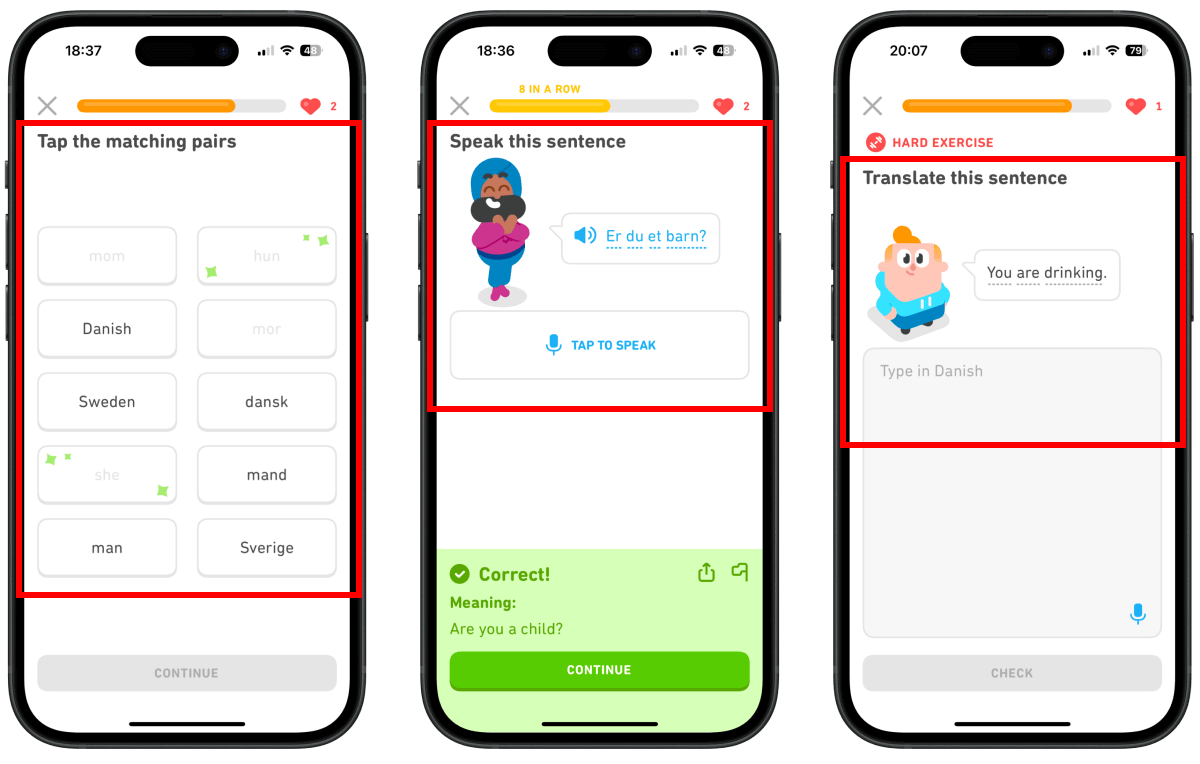
\includegraphics[width=0.98\textwidth]{src/figures/duolingo-exercise-types.png}
        \caption{Duolingo - Types of Exercises (highlighted in red)}
        \label{fig:duolingo-exercise-types}
    \end{figure}

    \item \textbf{Short Review After Finishing a Lesson}

    After completing each lesson, Duolingo presents users with an engaging summary screen accompanied by a celebratory animation (see Figure \ref{fig:duolingo-lesson-review}). The summary includes key metrics such as:

    \begin{itemize}
        \item Experience points (XP) earned
        \item Accuracy rate for the completed exercises
        \item Time spent practicing
        \item Maintenance of learning streaks
    \end{itemize}

    This immediate feedback loop is crucial for user motivation, as it provides a sense of achievement and progress tracking. The inclusion of XP points and streaks transforms the learning process into a game-like experience, encouraging users to maintain consistent practice habits. The celebratory animations and positive reinforcement help create a rewarding atmosphere, making the learning process more enjoyable.

    \begin{figure}[!h]
        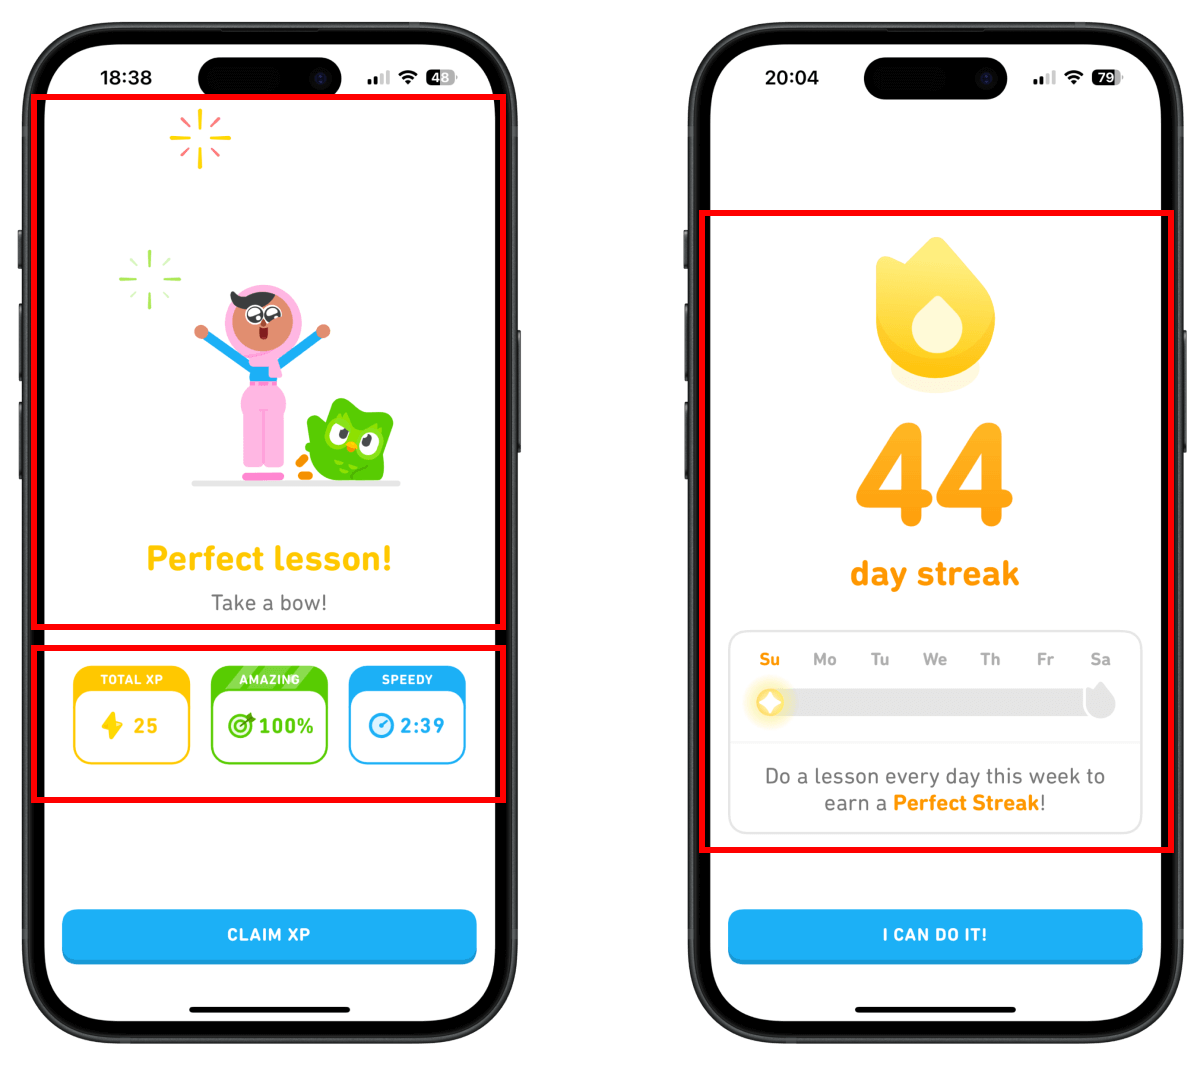
\includegraphics[width=0.85\textwidth]{src/figures/duolingo-lesson-review.png}
        \caption{Duolingo - Review After Finishing a Lesson (highlighted in red)}
        \label{fig:duolingo-lesson-review}
    \end{figure}

    \newpage

    \item \textbf{Daily Streak}

    One of Duolingo's most powerful gamification features is the daily streak system, which tracks consecutive days of learning activity (see Figure \ref{fig:duolingo-daily-streak}). Users maintain their streak by completing at least one lesson each day, creating a powerful psychological incentive for consistent practice. To make this system more flexible and user-friendly, Duolingo introduced "Streak Freezes" - items that users can acquire to preserve their streak during a day of inactivity.

    \begin{figure}[!h]
        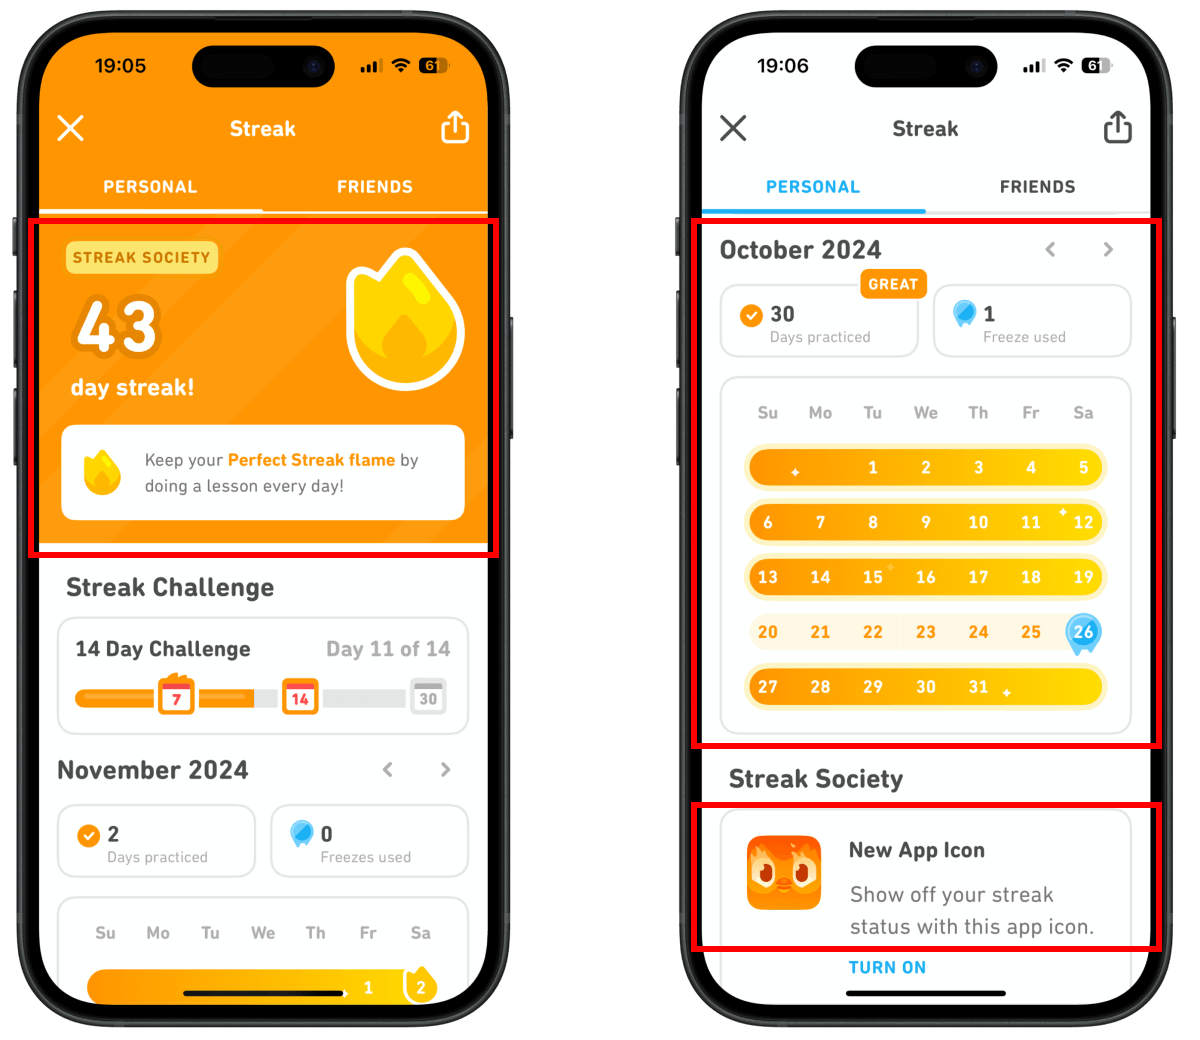
\includegraphics[width=0.72\textwidth]{src/figures/duolingo-streak.png}
        \caption{Duolingo - Daily Streak (highlighted in red)}
        \label{fig:duolingo-daily-streak}
    \end{figure}

    The streak system is supported by a sophisticated notification framework that employs various psychological triggers to maintain user engagement. These include:

    \begin{itemize}
        \item Reminder notifications at user-specified times
        \item Warnings when streaks are at risk of breaking
        \item Motivational messages to encourage streak continuation
        \item Interactive home screen widgets displaying streak counts
        \item Celebrations of streak milestones
        \item Collectible app icons that unlock at different streak milestones
    \end{itemize}

    These features work together to create multiple touchpoints throughout the user's day, combining immediate rewards with long-term achievement tracking. The effectiveness of this approach is evident in the data. Over 20\% of Duolingo's daily active users maintain streaks longer than one year \cite{cite:duolingo_2024q2}. The streak system exemplifies how gamification can transform a learning obligation into an engaging daily ritual, effectively addressing one of language learning's most significant challenges: maintaining a consistent practice.
    
\end{itemize}

\section{Comparison and Findings}

The analysis of gamification features across English Mind and similar applications reveals several interesting patterns and opportunities for enhancement. Table \ref{tab:gamification-comparison} provides a comprehensive overview of the features implemented across all analyzed applications, highlighting both commonalities and unique approaches.

\begin{table}[h]
    \caption{Comparison of Gamification Features Across Applications}
    \label{tab:gamification-comparison}
    
    % Spacing between rows and columns
    \renewcommand{\arraystretch}{1.2}
    \setlength{\tabcolsep}{2pt}
    
    \begin{tabular}{l>{\centering}p{2cm}>{\centering}p{2cm}>{\centering}p{2cm}>{\centering\arraybackslash}p{2cm}}
        \toprule
        \textbf{Feature} & \textbf{English Mind} & \textbf{WordUp} & \textbf{DuoCards} & \textbf{Duolingo} \\
        \midrule
        \multicolumn{5}{l}{\textbf{Flashcard Variations}} \\
        Multiple flashcard types & \textemdash & \ding{51} & \ding{51} & \ding{51} \\
        Spelling exercises & \textemdash & \ding{51} & \ding{51} & \ding{51} \\
        Matching exercises & \textemdash & \ding{51} & \ding{51} & \ding{51} \\
        Speaking exercises & \textemdash & \textemdash & \textemdash & \ding{51} \\
        \midrule
        \multicolumn{5}{l}{\textbf{Progress Tracking}} \\
        Overall progress visualization & \ding{51} & \ding{51} & \ding{51} & \ding{51} \\
        Practice session progress bar & \ding{51} & \ding{51} & \ding{51} & \ding{51} \\
        Individual word progress & \textemdash & \ding{51} & \textemdash & \textemdash \\
        \midrule
        \multicolumn{5}{l}{\textbf{Streaks and Daily Goals}} \\
        Streak system & \textemdash & \textemdash & \ding{51} & \ding{51} \\
        Daily word goal & \ding{51} & \textemdash & \textemdash & \textemdash \\
        Daily time goal & \textemdash & \ding{51} & \textemdash & \textemdash \\
        \midrule
        \multicolumn{5}{l}{\textbf{Rewards and Motivation}} \\
        Virtual currency & \textemdash & \textemdash & \ding{51} & \ding{51} \\
        Post-practice review & \textemdash & \textemdash & \textemdash & \ding{51} \\ 
        Leaderboards & \textemdash & \ding{51} & \textemdash & \ding{51} \\
        Mascot upgrade system & \textemdash & \textemdash & \ding{51} & \textemdash \\
        \bottomrule
    \end{tabular}
\end{table}

Key findings from the analysis include:

\begin{itemize}
    \item \textbf{Flashcard Variation is Standard}
    
    WordUp, DuoCards, and Duolingo all incorporate multiple types of exercises or flashcards, contrasting with English Mind's current single-format approach. This variety helps prevent learning fatigue and addresses different aspects of vocabulary acquisition. Particularly noteworthy is Duolingo's integration of speaking exercises, which could become more feasible with advancing language processing technologies.

    \item \textbf{Basic Progress Tracking is Universal}
    
    All analyzed applications implement some form of progress visualization, suggesting this is a fundamental gamification feature for vocabulary learning apps. However, WordUp's individual word progress tracking stands out as a unique approach that could enhance user engagement with specific vocabulary items.

    \item \textbf{Diverse Approaches to Daily Goals}
    
    While all applications encourage regular practice, they employ different strategies. English Mind focuses on word quantity goals, whereas WordUp emphasizes time-based goals. Duolingo's streak system, supported by its comprehensive notification framework and streak freeze mechanism, appears particularly effective at maintaining long-term user engagement.

    \item \textbf{Reward Systems Vary}
    
    The analysis reveals diverse approaches to reward systems. DuoCards' mascot upgrade system and virtual currency provide tangible rewards for learning progress, while WordUp's leaderboard system adds a social competitive element. Duolingo combines multiple approaches, including post-practice reviews and virtual currency. English Mind currently lacks such reward mechanisms, presenting an opportunity for enhancement.

\end{itemize}

These findings suggest several potential areas for improving English Mind's gamification framework:

\begin{enumerate}
    \item \textbf{Flashcard Diversification:} Implementing various flashcard types could make practice sessions more engaging while reinforcing learning through different approaches.
    
    \item \textbf{Enhanced Progress Tracking:} Adding individual word progress tracking could provide users with more detailed insights into their learning journey.
    
    \item \textbf{Engagement Mechanisms:} Introducing a streak system with protective features (like streak freezes) could encourage consistent practice habits.
    
    \item \textbf{Reward Framework:} Developing a reward system, whether through virtual currency, achievements, or social features, could provide additional motivation for continued engagement.
\end{enumerate}

These improvements should be carefully designed to complement English Mind's existing learning methodology while enhancing user engagement and motivation. The next chapter will explore specific recommendations for implementing these enhancements.